% !Rnw root = learnR.Rnw




\section{Fine tuning the installation}\label{sec:fine-tune}
The information in this section is relevant mainly to users of the Windows
or Mac GUI, rather than RStudio.  With RStudio, work is typically
organized by projects, albeit usually with a different working
directory for each different project.

\begin{figure*}
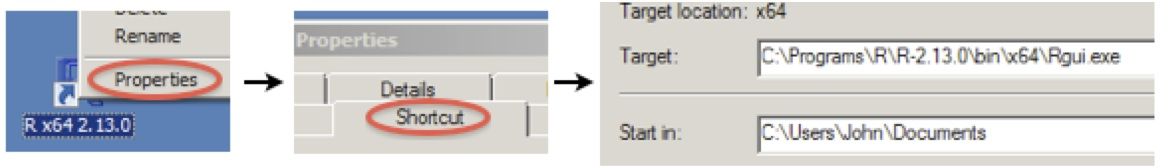
\includegraphics{figs-inc/16i-gui-prop.jpg}
\caption{This shows the sequence of clicks needed to display the
page from which the \underline{Start in:} directory can be set. This
will then be the working directory in which R will start.\label{fig:startin}}
\end{figure*}

\paragraph{The working directory:}  This is best set to a directory that is
convenient for storing files connected with the project on which you are
currently working.  When starting a new project, it to start
a new working directory.

Under Windows, each R icon has associated with it a working directory.
\marginnote{Under MacOS X, dragging a file onto the R icon will start
  R in the directory that contains the file.  Alternatively,
  in a terminal window, type for example:\\
  \margtt{open -a R $\sim$/r/course}\\
  \noindent This will start R with {\bf \ensuremath{\sim}/r/course} as
  working directory.}  Right click the icon.  Then click on
\underline{Properties} (at the bottom of the list), thus displaying
the Properties submenu.  Make sure that \underline{Shortcut} is
selected.  Set the \underline{Start in:} directory to the working
directory in which you want R to start.  See Figure \ref{fig:startin}.

\paragraph{Multiple (MDI) or Single (SDI) display interface for Windows:}
One way to get R to start in SDI mode is to add \texttt{--sdi}, with a
preceding space, to the target that is shown in Figure
\ref{fig:startin}.

\section{Setting the Default CRAN Mirror}\label{sec:mirror}
The default CRAN mirror can be set from the Windows or MacOS X R GUI.\\[-3pt]

\begin{figure}[h]
\noindent {\em Windows:} Click on \underline{Packages} $\mid$ \underline{Set CRAN mirror \ldots}\\[6pt]
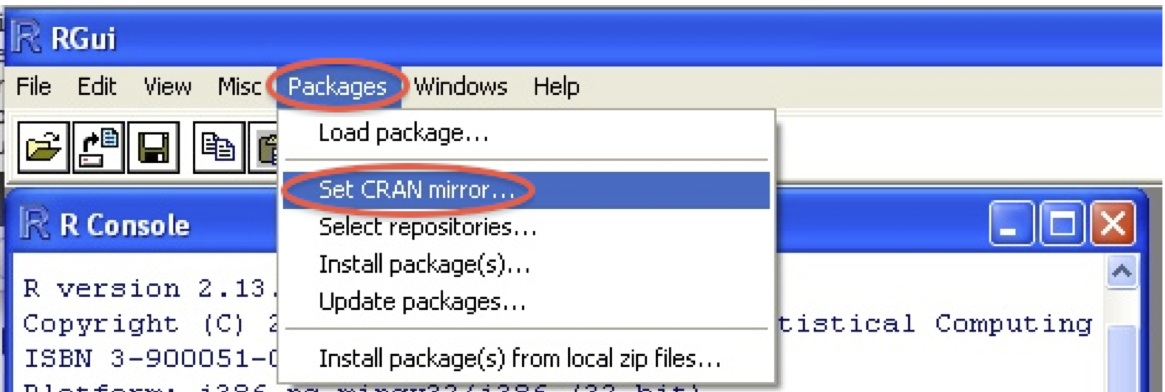
\includegraphics{figs-inc/16i-win-mirrors.jpg}
\caption{This shows the R Windows GUI menu option that can be used to
  set the CRAN mirror.  If not set, the user is asked to nominate the
  mirror whenever one or more packages are downloaded or updated from
  CRAN.}
\end{figure}
\vspace*{-18pt}


% \noindent{{\em MacOSX:} Click on \underline{R} $\mid$ \underline{Preferences}}

\noindent
\begin{figure}[h]
\noindent {\em MacOS X:} Click on \underline{R} $\mid$ \underline{Preferences}\\
\begin{minipage}[t]{0.31\textwidth}
\vspace*{0pt}

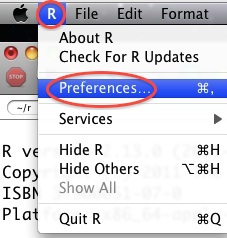
\includegraphics{figs-inc/16i-mac-rprefs.jpg}

Click on \underline{Preferences}.  Then click, if necessary, on
\underline{Startup} to display the startup options, shown in the
Window on the right.
\end{minipage}
\hspace*{0.02\textwidth}
\begin{minipage}[t]{0.655\textwidth}
\vspace*{0pt}

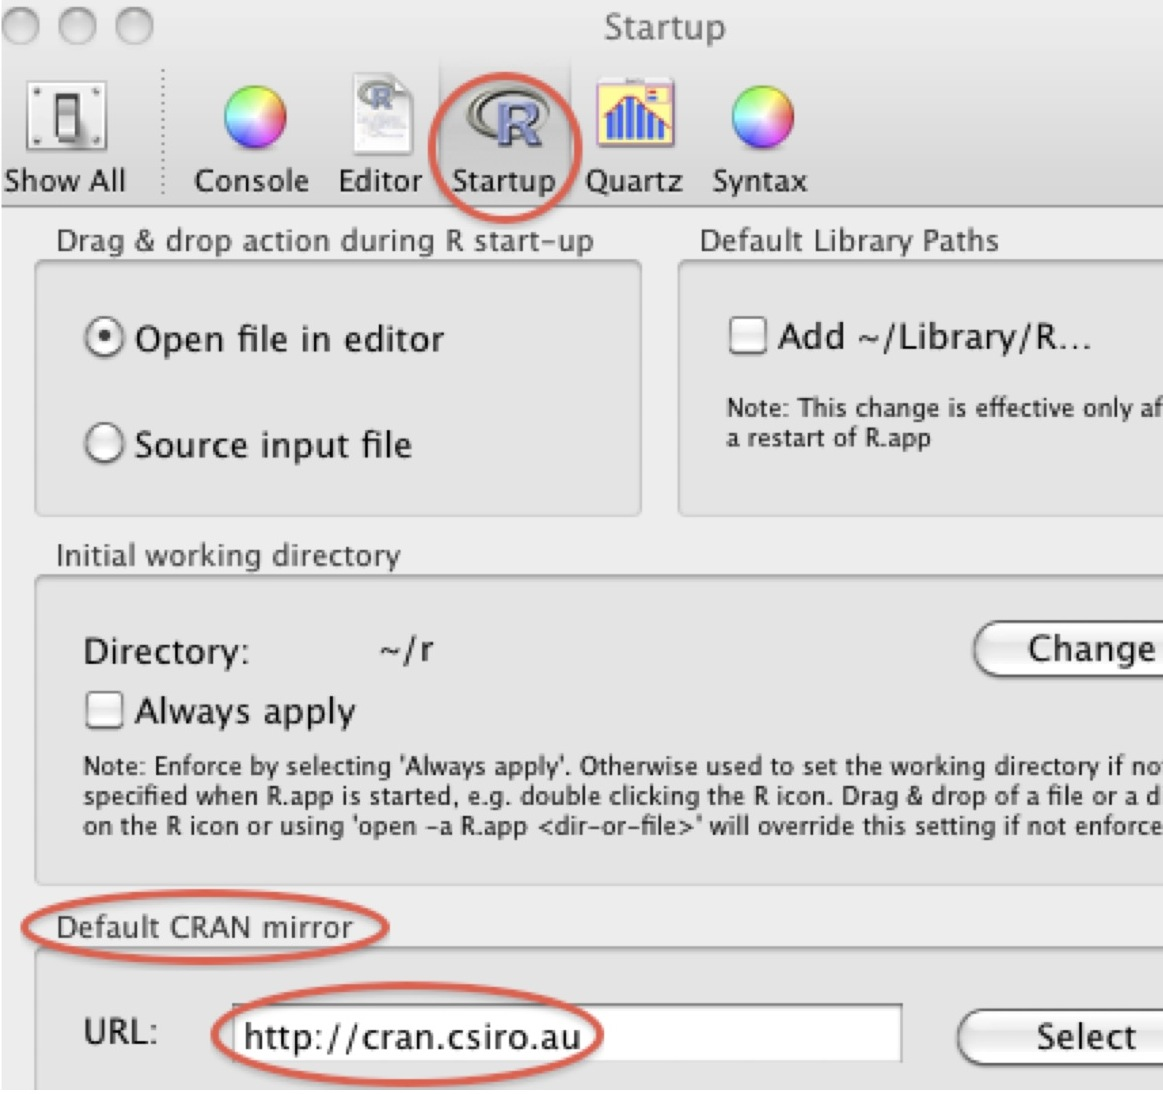
\includegraphics{figs-inc/16i-mac-rstartup.jpg}
\end{minipage}
\caption{In a factory fresh MacOS X installation, packages are
  downloaded from \url{http://cran.r-project.org}.  The preferences
  pages allow the setting of a wide variety of other preferences
  also.}
\end{figure}

\section{R system information}

If access is needed to files that are in the R installation tree,
obtain the path, thus:
\begin{Schunk}
\begin{Sinput}
R.home()
\end{Sinput}
\begin{Soutput}
[1] "C:/PROGRA~1/R/R-32~1.2"
\end{Soutput}
\end{Schunk}
When using Microsoft Windows systems, a more intelligible result is
obtained by wrapping the function call in \txtt{normalizePath()},
thus: \marginnote{If the \margtt{winslash="/"} argument is omitted,
  double backslashes are used to separate names in the directory
  tree.}
\begin{Schunk}
\begin{Sinput}
normalizePath(R.home(), winslash="/")
\end{Sinput}
\begin{Soutput}
[1] "C:/Program Files/R/R-3.2.2"
\end{Soutput}
\end{Schunk}

To see a list of all R system variables, type
\begin{Schunk}
\begin{Sinput}
names(Sys.getenv())
\end{Sinput}
\end{Schunk}
These can then be inspected individually.
\begin{Schunk}
\begin{Sinput}
Sys.getenv("R_HOME")
\end{Sinput}
\begin{Soutput}
[1] "C:/PROGRA~1/R/R-32~1.2"
\end{Soutput}
\end{Schunk}
See \txtt{help(Rprofile)} for details on how to set system variables.

The following can be used to get the path to files that come with an installed
package:
\begin{fullwidth}
\begin{Schunk}
\begin{Sinput}
system.file("misc/ViewTemps.RData", package="DAAG")
\end{Sinput}
\begin{Soutput}
[1] "C:/Users/JohnM/Documents/R/win-library/3.2/DAAG/misc/ViewTemps.RData"
\end{Soutput}
\end{Schunk}
\end{fullwidth}

\section{Repositories additional to CRAN}\label{sec:repos}

Figure \ref{fig:repos} shows a list of available repositories, as given by
the Windows GUI, after clicking on:
\txtt{\underline{Packages}}\txtt{|}\txtt{\underline{Set repositories}}.
To select more than one repository, hold down the Windows key, or
under MacOS X the command key, while left-clicking.

\begin{marginfigure}
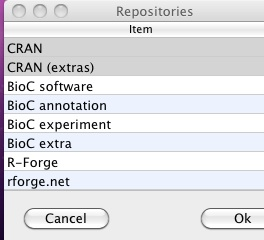
\includegraphics{figs-inc/16i-repos.jpg}
\caption{List of available repositories, as given by the Windows
  GUI.}\label{fig:repos}
\end{marginfigure}

To use the command line to view a list of all repositories known to the R
installation, and possibly to select one or more, type:
\begin{Schunk}
\begin{Sinput}
setRepositories()
\end{Sinput}
\end{Schunk}
Alternatively, use the argument \txtt{ind}, in a call to
\txtt{setRepositories()}, to specify repositories.  For example:
\begin{Schunk}
\begin{Sinput}
setRepositories(ind=1:2)
\end{Sinput}
\end{Schunk}

\section{Running R in Batch Mode}

\marginnote{For Windows 64-bit R (2.12.0 or later), the directory {\bf
  R\_HOME$\boldsymbol{\backslash}$bin$\boldsymbol{\backslash}$x64}
must be in the system path. For Windows 32-bit R, replace {\bf x64}
by {\bf i386}. For determining {\bf R\_HOME}, see above.}

On the command line (for Windows, Unix, Linux, \ldots), enter
\begin{verbatim}
R CMD BATCH infile outfile
\end{verbatim}

Here infile is a file that holds R commands.  See \txtt{help(BATCH)}
for further information. The path to the R executable must be included
in the system path variable. The R FAQ for Windows has information on
setting environment variables.

\section{The R Windows installation directory tree}

The R system can be installed into any directory where the installer
has write permission.  The hierarchy of directories and files that
form the R installation is termed the \textit{directory tree}.  Likely
defaults for the directory tree of an R-3.2.2 Windows installation are:\\
{\small \textbf{C:$\boldsymbol{\backslash}$PROGRAM FILES$\boldsymbol{\backslash}$R$\boldsymbol{\backslash}$R-3.2.2$\boldsymbol{\backslash}$}}\\
\noindent or, for example,\\
{\small \textbf{C:$\boldsymbol{\backslash}$Documents and
  Settings$\boldsymbol{\backslash}$Owner$\boldsymbol{\backslash}$My
  Documents$\boldsymbol{\backslash}$R$\boldsymbol{\backslash}$R-3.2.2$\boldsymbol{\backslash}$}}

The directory tree is relocatable.  It can be copied to a flash drive
or CD or DVD, which can be then be used to run R.
\marginnote{For running R from a DVD (or CD), be sure to change the
\underline{Start In} directory to a directory that is writable.}
Thus, copy the installation tree with root at
\textbf{C:$\boldsymbol{\backslash}$Program
  Files$\boldsymbol{\backslash}$R$\boldsymbol{\backslash}$R-3.2.2$\boldsymbol{\backslash}$}
across to \textbf{D:} to become a tree with root
\textbf{D:$\boldsymbol{\backslash}$R-3.2.2$\boldsymbol{\backslash}$}.
The executable (binary)
\textbf{D:$\boldsymbol{\backslash}$R-3.2.2$\boldsymbol{\backslash}$bin$\boldsymbol{\backslash}$x64$\boldsymbol{\backslash}$Rgui.exe}
can then be used to start a 64-bit R session. To verify that this works,
click on its icon.
For 32-bit R, replace {\bf x64}, where it appears in the path, by {\bf i386}.

\section{Library directories}
Packages that the user installs can go anywhere on the system.
It is not necessary to install them into the library directory
that is in the R directory tree.

An R session that is running from one installation, perhaps the main
installation on the hard drive, can in principle access any compatible
R library directory that is available.  Thus, the
following gives access, from an R session that is started (e.g.) from
the hard drive, to to a library tree that is stored under
\textbf{D:$\boldsymbol{\backslash}$R-3.2.2}:
\begin{Schunk}
\begin{Sinput}
.libPaths("D:/R-3.0.2/library")
\end{Sinput}
\end{Schunk}
\noindent
This might for example be the library tree from an R installation on a
DVD that has been placed in the \textbf{D:} drive.

To avoid the need to type this each time a new session is started in
that working directory, create the following function:\sidenote{This
  function will then be saved as part of the default workspace, and
  executed at the start of any new session in that directory.}
\begin{Schunk}
\begin{Sinput}
.First <- function().libPaths("D:/R-3.0.2/library")
\end{Sinput}
\end{Schunk}
\noindent
Alternatively, the function can be placed in a startup profile file,
as described in the next section.

In moving to a new major version of R (e.g., from R-3.1.2 to
R-3.2.0), the library directory in the R installation tree is
replaced.  A relatively painless way to update the new installation
library directory is to copy packages across from the former
installation library directory to the new library directory, being
careful not to replace any existing packages in that directory.  (If
of course packages are in a separate user directory, no moving is
required.)  Then, from within R, type:
\begin{Schunk}
\begin{Sinput}
update.packages(checkBuilt=TRUE, ask=FALSE)
## Check package status:
summary(packageStatus())
\end{Sinput}
\end{Schunk}

Use of a {\bf .Renviron} file in the home directory is a further
possibility. This can be conveniently done from within R:\sidenote{This
follows a suggestion from Bill Venables.}
\begin{Schunk}
\begin{Sinput}
cat('LIB1="C:/Users/owner/R/win-library/2.15"\n',
    file = "~/.Renviron", append = TRUE)
cat('LIB2="C:/Users/owner/R/win-library/2.14"\n',
    file = "~/.Renviron", append = TRUE)
cat('LIB1="R_LIBS_USER=${LIB1};${LIB2}\n',
    file = "~/.Renviron", append = TRUE)
\end{Sinput}
\end{Schunk}

\section{The Startup mechanism}

Various system variables are set at startup, and a number of packages
are attached.  The details can be controlled at an installation level,
at a user level, and at a startup directory level.  If started in the
standard manner, the 'R\_PROFILE' environment variable\footnote{If
  this is unset, R searches for a file {\bf
    R\_HOME/etc/Rprofile.site}.  'Factory-fresh' installations will
  not have such a file.  Code is sourced into the \textit{base}
  package, before other packages are loaded.} can be used to give the
name of a site-wide profile file.  See \txtt{help(Startup)} for
details.

R next searches at startup for a file called \textbf{.Rprofile} in the
current directory or in the user's home directory (in that
order).\sidenote{Alternatively, the 'R\_PROFILE\_USER' environment variable
can be used to set the name of a user profile file.}
Such a \textbf{.Rprofile} file can for example define a
\txtt{.First()} and/or a \txtt{.Last()} function.

A user (or site-wide) profile file might for example include the
following statements:
\begin{Schunk}
\begin{Sinput}
options(papersize="a4")
options(editor="notepad")         # Preferred editor
options(pager="internal")
options(tab.width = 4)
options(width = 120)              # Wider console line
options(graphics.record=TRUE)
options(show.signif.stars=FALSE)  # Banish the stars
options(prompt="? ")              # Use '?' as prompt
options(continue="  ")            # Blank continuation
.libPaths("C:/my_R_library")      # Add library to path.
\end{Sinput}
\end{Schunk}
